%-------------------------------------------
\begin{frame}[containsverbatim]
\frametitle{Practical exercise}
%-------------------------------------------
\begin{exampleblock}{}
For this practical exercise on Snakemake we will:
\begin{itemize}
    \item access to conda by the way of a docker container
    \item access to snakemake and analysis tools by the way of a conda environment (details about conda will be seen after)
    \item create a first snakefile with one rule
    \item add a second rule to create a first workflow
\end{itemize}
\end{exampleblock}
During this first exercise, we will execute several cycles: executing snakemake, observing the result and improving the code. Each code version will be noted \verb|ex1_oX.smk| with X a progressive digit.\\
(or save on github ...)
\end{frame}
%-------------------------------------------
\begin{frame}
\frametitle{Practical exercise}
%-------------------------------------------
\begin{columns}
 \column{0.35\textwidth}
 The final objective is to create a snakefile to manage this small workflow:
   \begin{exampleblock}{a small workflow}
   \begin{center}
       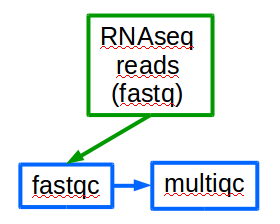
\includegraphics[width=3.5cm]{03_workflow/images/FAIR_WF_2steps.png}
   \end{center}
   \end{exampleblock}

 \column{0.55\textwidth}
   \begin{exampleblock}{Input data}
    The input data, the RNASeq reads files, may be downloaded from: \url{https://zenodo.org/record/3997237}
    \begin{center}
        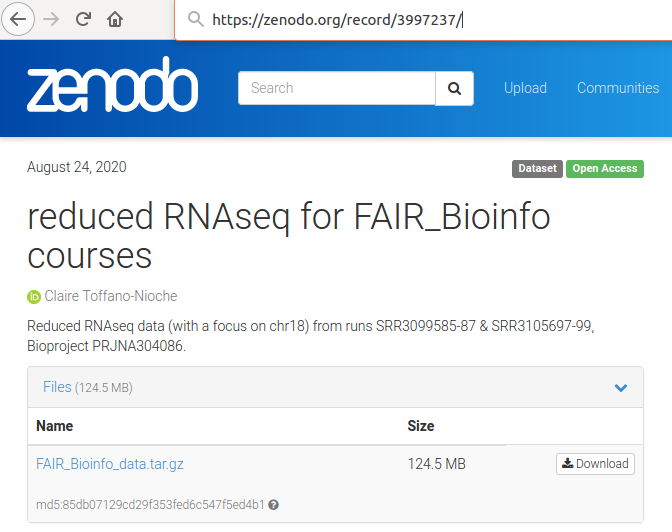
\includegraphics[width=5cm]{03_workflow/images/FAIR_data_zenodo.png}
    \end{center}
   Download and unzip
   \end{exampleblock}
\end{columns}
\end{frame}
%-------------------------------------------
\begin{frame}[containsverbatim]
\frametitle{Exercise setup}
%-------------------------------------------
We will access to the analysis tools thanks to a conda environment, \verb|envfair.yml| (cf. next slide), designed for this small workflow:
\begin{exampleblock}{Conda environment}
\begin{lstlisting}[language=python]
# do go to the parent directory of Data (from the downloaded and unziped data):
cd ......
# create envfair.yml
\end{lstlisting}
\end{exampleblock}
We will access to Snakemake by running a docker image containing the conda tool:
\begin{exampleblock}{Docker miniconda3}
\begin{lstlisting}
docker run -it -v ${PWD}:/data continuumio/miniconda3
cd data
conda env create -n envfair -f envfair.yml
conda activate envfair
\end{lstlisting}
\end{exampleblock}
\end{frame}
%-------------------------------------------
\begin{frame}[containsverbatim]
\frametitle{Exercise setup}
%-------------------------------------------
\begin{exampleblock}{envfair.yml}
\begin{lstlisting}[language=python]
channels:
  - conda-forge
  - bioconda
  - default
dependencies:
  # workflow manager:
  - bioconda::snakemake-minimal>=6.5 
  # check quality of fastq data (java)
  - bioconda::fastqc=0.11.9 
  # R package to aggregate reports
  - bioconda::multiqc=1.9 
\end{lstlisting}
\end{exampleblock}
\end{frame}
%-------------------------------------------
\begin{frame}[containsverbatim]
\frametitle{Rule concept with one input file}
%-------------------------------------------
\begin{exampleblock}{Objective 1}
Create a snakemake file named \verb|ex1_o1.smk| including the first step of the RNAseq workflow (the reads quality checking thank to the \verb|fastqc| tool) on one of the RNAseq files
\end{exampleblock}
\begin{exampleblock}{Hint}
\begin{itemize}
    \item input file: \verb|SRR3099585_chr18.fastq.gz| in a local directory of yours
    \item fastqc access: by running \verb|docker miniconda3| + activate the conda \verb|envfair| environment
    \item fastqc command: \verb|fastqc inputFileName --outdir FastQCResultDirectory|
    \item the 2 fastqc result files (\verb|*_fastqc.zip| \& \verb|*_fastqc.html|) will be located in the fastqc result directory and will be named based on the prefix of input file (eg. \verb|SRR3099585_chr18_fastqc.zip|)
\end{itemize}
\end{exampleblock}
\end{frame}
%-----------------------------------------------
\begin{frame}[containsverbatim]
\frametitle{Solution}
%-------------------------------------------
\begin{exampleblock}{ex1$\_$o1.smk}
\begin{lstlisting}[language=python]
rule fastqc:
  output:
    "FastQC/SRR3099585_chr18_fastqc.zip", 
    "FastQC/SRR3099585_chr18_fastqc.html"
  input:
    "Data/SRR3099585_chr18.fastq.gz"
  shell: "fastqc --outdir FastQC/ {input}"
\end{lstlisting}
\end{exampleblock}
\begin{exampleblock}{Snakemake run}
\begin{lstlisting}[language=python]
snakemake --cores 1 --snakefile ex1_o1.smk
\end{lstlisting}
\end{exampleblock}
\begin{exampleblock}{Observe result}
Look at the newly created \verb|FastQC| directory: Snakemake create alone the needed directories.
\end{exampleblock}
\end{frame}
%-------------------------------------------
\begin{frame}[containsverbatim]
\frametitle{One rule, 2 input files}
%-------------------------------------------
\begin{exampleblock}{Objective 2}
Add a second input RNAseq file to the rule
\end{exampleblock}
\begin{exampleblock}{Hint}
\begin{itemize}
    \item input file: \verb|SRR3099586_chr18.fastq.gz| in a local directory of yours
    \item don't forget the output files
\end{itemize}
\end{exampleblock}
\end{frame}
%-----------------------------------------------
\begin{frame}[containsverbatim]
\frametitle{Solution}
%-------------------------------------------
\begin{exampleblock}{ex1$\_$o2.smk}
\begin{lstlisting}[language=python]
rule fastqc:
  output:
    "FastQC/SRR3099585_chr18_fastqc.zip", 
    "FastQC/SRR3099585_chr18_fastqc.html",
    "FastQC/SRR3099586_chr18_fastqc.zip", 
    "FastQC/SRR3099586_chr18_fastqc.html"
  input:
    "Data/SRR3099585_chr18.fastq.gz",
    "Data/SRR3099586_chr18.fastq.gz"
  shell: "fastqc --outdir FastQC/ {input}"
\end{lstlisting}
\end{exampleblock}
\begin{exampleblock}{Snakemake run}
\begin{lstlisting}[language=python]
snakemake -c1 -s ex1_o2.smk
# -s & -c: short forms of the --snakefile & --cores options
\end{lstlisting}
\end{exampleblock}
\end{frame}
%-------------------------------------------
\begin{frame}[containsverbatim]
\frametitle{Solution}
%-------------------------------------------
\begin{exampleblock}{Observe result}
Snakemake run the fastqc tool only for the 2nd input file added. 
\end{exampleblock}

\begin{exampleblock}{Run again}
Run again the snakemake command: \verb|snakemake -c1 -s ex1_o2.smk|\\

Why does Snakemake reply \verb|"Nothing to be done"|?
\end{exampleblock}

\begin{exampleblock}{Solutions}
\begin{itemize}
   \item delete the FastQC directory (\verb|rm -Rf FastQC|) and rerun the snakemake command
   \item use the Snakemake \verb|--forcerules| (\verb|-R|) option: \verb|snakemake -c1 -s ex1_o2.smk -R fastqc|
\end{itemize}
\end{exampleblock}
\end{frame}
%-------------------------------------------
\begin{frame}[containsverbatim]
\frametitle{Manage all the RNAseq files}
%-------------------------------------------
\begin{exampleblock}{Objective 3}
Add all the RNAseq files.\\
Boring with writing all input and output file names? \\
Use the \verb|expand()| function to manage all the input RNAseq files at once.
\end{exampleblock}
\begin{exampleblock}{Hint}
\begin{itemize}
    \item create a Python list at the begining of the snakefile and containing all the basename of the input files (don't include the "\verb|.fastq.gz|" suffix).\\
    Python list: \verb|list_name = ["item1", "item2", ..., "itemN"]|
    \item replace the filename lists of the input and output directives by the \verb|expand()| function
\end{itemize}
\end{exampleblock}
\end{frame}
%-----------------------------------------------
\begin{frame}[containsverbatim]
\frametitle{Solution}
%-------------------------------------------
\begin{exampleblock}{ex1$\_$o3.smk}
\begin{lstlisting}[language=python]
SAMPLES = ["SRR3099585_chr18","SRR3099586_chr18","SRR3099587_chr18"] # add all 6 samples

rule fastqc:
  output:
    expand("FastQC/{sample}_fastqc.zip", sample = SAMPLES),
    expand("FastQC/{sample}_fastqc.html", sample = SAMPLES)
  input:
    expand("Data/{sample}.fastq.gz", sample = SAMPLES)
  shell: "fastqc --outdir FastQC/ {input}"
\end{lstlisting}
\end{exampleblock}
\begin{exampleblock}{Snakemake run}
\begin{lstlisting}[language=python]
rm -Rf FastQC/
snakemake -c1 -s ex1_o3.smk
\end{lstlisting}
\end{exampleblock}
\end{frame}
%-----------------------------------------------
\begin{frame}[containsverbatim]
\frametitle{Add a second rule}
%-----------------------------------------------
\begin{exampleblock}{Objective 4}
Add a second rule: this will start a workflow. \\
The second tool/rule will aggregate all the fastqc results thank to the R multiqc tool. 
\end{exampleblock}
\begin{exampleblock}{Hint}
\begin{itemize}
    \item inputs: the fastqc zip files
    \item command: \verb|multiqc FastQCResultDirectory|
    \item 2 outputs: a file \verb|multiqc_report.html| \& a repository \verb|multiqc_data|
\end{itemize}
\end{exampleblock}
\end{frame}
%-----------------------------------------------
\begin{frame}[containsverbatim]
\frametitle{Solution}
%-------------------------------------------
\begin{exampleblock}{ex1$\_$o4.smk (copy, run)}
\begin{lstlisting}[language=python]
SAMPLES = ["SRR3099585_chr18","SRR3099586_chr18","SRR3099587_chr18"]

rule fastqc:
  output:
    expand("FastQC/{sample}_fastqc.zip", sample = SAMPLES),
    expand("FastQC/{sample}_fastqc.html", sample = SAMPLES)
  input:
    expand("Data/{sample}.fastq.gz", sample = SAMPLES)
  shell: "fastqc --outdir FastQC/ {input}"

rule multiqc:
  output:
    "multiqc_report.html",
    directory("multiqc_data")
  input:
    expand("FastQC/{sample}_fastqc.zip", sample = SAMPLES)
  shell: "multiqc {input}"
\end{lstlisting}
\end{exampleblock}
%\begin{exampleblock}{Snakemake run}
%\begin{lstlisting}[language=python]
%snakemake -c1 -s ex1_o4.smk
%\end{lstlisting}
%\end{exampleblock}
\end{frame}
%-------------------------------------------
\begin{frame}[containsverbatim]
\frametitle{Solution}
%-------------------------------------------
\begin{exampleblock}{Observe result}
Does Snakemake do the job?\\
Why wasn't the fastqc command launched?\\
\end{exampleblock}
\begin{exampleblock}{rule links}
Snakemake run the first rule (fastqc) and stop when the target files are present. \\
Solutions ?\begin{itemize}
    \item put the multiqc rule before the fastqc rule
    \item add a rule that aggregate all the rules of the workflow
\end{itemize} 
Adding a new rule is the choice (could be no link between the rules)
\end{exampleblock}
\end{frame}
%-------------------------------------------
\begin{frame}[containsverbatim]
\frametitle{The target rule}
%-------------------------------------------
\begin{exampleblock}{Objective 5}
Add a "first" rule (named "all", "target", ...) with the expected results for all the rules in its \verb|input:| directive.
\end{exampleblock}
\end{frame}
%-------------------------------------------
\begin{frame}[containsverbatim]
\frametitle{Solution}
%-------------------------------------------
\begin{exampleblock}{ex1$\_$o5.smk}
\begin{lstlisting}
...
rule all:
  input:
    expand("FastQC/{sample}_fastqc.html", sample=SAMPLES),
    "multiqc_report.html",
    directory("multiqc_data")
...
\end{lstlisting}
\end{exampleblock}
\begin{exampleblock}{Snakemake run}
\begin{lstlisting}[language=python]
snakemake -c1 -s ex1_o5.smk -R fastqc
\end{lstlisting}
\end{exampleblock}
\end{frame}
%-------------------------------------------
\begin{frame}[containsverbatim]
\frametitle{Solution}
%-------------------------------------------
\begin{exampleblock}{Observe result}
Does Snakemake do the job?\\
\end{exampleblock}
\begin{exampleblock}{Fastqc: job or jobs?}
Look at more precisely the fastqc job. We have many input files but snakemake launched only one fastqc job:
\begin{center}
    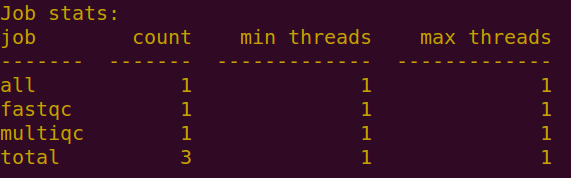
\includegraphics[width=6cm]{03_workflow/images/FAIR_ex1_o5_smk.png}
\end{center}
It is because the \verb|fastqc| rule is defined with a list of files and not for one unique file and because the \verb|fastqc| tool accepts both a unique file as well as a list of files.
\end{exampleblock}
\end{frame}
%-------------------------------------------
\begin{frame}[containsverbatim]
\frametitle{Running n individual jobs}
%-------------------------------------------
\begin{exampleblock}{Objective 6}
Thank to the \verb|all| rule, all expected files are designated. So we don't need to give the \verb|fastqc| rule a list anymore and we can replace it to manage only one file and all files one by one. We will gain in power in systems having more than one core.
\end{exampleblock}
\begin{exampleblock}{Hint}
Replace the \verb|expand()| function with a simple wildcard for the filename in the \verb|fastqc| rule.
\end{exampleblock}
\end{frame}
%-------------------------------------------
\begin{frame}[containsverbatim]
\frametitle{Solution}
%-------------------------------------------
\begin{exampleblock}{ex1$\_$o6.smk}
\begin{lstlisting}
rule fastqc:
  output:
    "FastQC/{sample}_fastqc.zip",
    "FastQC/{sample}_fastqc.html"
  input:
    "Data/{sample}.fastq.gz"
  shell: "fastqc --outdir FastQC/ {input}"
\end{lstlisting}
\end{exampleblock}
\begin{exampleblock}{Snakemake run}
\begin{lstlisting}[language=python]
snakemake -c1 -s ex1_o6.smk -R fastqc
\end{lstlisting}
\end{exampleblock}
\end{frame}
%-------------------------------------------
\begin{frame}[containsverbatim]
\frametitle{Solution}
%-------------------------------------------
\begin{exampleblock}{Observe result}
Now Snakemake did many fastqc jobs:
\begin{center}
    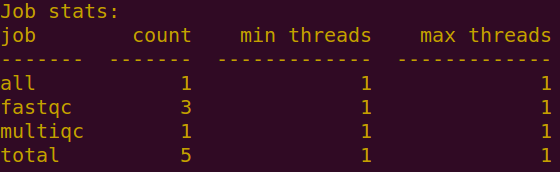
\includegraphics[width=6cm]{03_workflow/images/FAIR_ex1_o6_smk.png}
\end{center}
\end{exampleblock}
\begin{exampleblock}{Parallelize}
Rerun with more than one core: 
\begin{lstlisting}[language=python]
snakemake -c3 -s ex1_o6.smk -R fastqc
\end{lstlisting}
What happens now to the runtime displays on the screen?\\

To correct the mixture, we will move the displays to a log file specific for each rule and each input file.
\end{exampleblock}
\end{frame}
%-------------------------------------------
\begin{frame}[containsverbatim]
\frametitle{Adding log file}
%-------------------------------------------
\begin{exampleblock}{Objective 7}
In Unix systems, the output of a command is usually sent to 2 separate streams: the expected output to Standard Out (stdout, or "\verb|>|"), and the error messages to Standard Error (stderr, or "\verb|2>|"). \\
To integrate stderr and stdout into the same log, use "\verb|&>|". But use it with care because output files are often printed to stdout.
\end{exampleblock}
\begin{exampleblock}{Hint}
Redirect the stdout and stderr streams of the \verb|fastqc| and \verb|multiqc|  rules by adding a "\verb|log:|" directive with two variables, \verb|out| and \verb|err| to separately redirect each streams.
\end{exampleblock}
\end{frame}
%-----------------------------------------------
\begin{frame}[containsverbatim]
\frametitle{Solution}
%-------------------------------------------
\begin{exampleblock}{ex1$\_$o7.smk}
\begin{lstlisting}[language=python]
# in rule multiqc:
  log:
    out="Logs/multiqc.std",
    err="Logs/multiqc.err"
  shell: "multiqc {input} 1>{log.std} 2>{log.err}"
# in rule fastqc:
  log:
    log1="Logs/{sample}_fastqc.log1",
    log2="Logs/{sample}_fastqc.log2"
  shell: "fastqc --outdir FastQC/ {input} 1>{log.log1} 2>{log.log2}"
\end{lstlisting}
\end{exampleblock}
\begin{exampleblock}{Snakemake run}
\begin{lstlisting}[language=python]
snakemake -c1 -s ex1_o7.smk -R fastqc
\end{lstlisting}
\end{exampleblock}
\end{frame}